% \setcounter{page}{1}
\begin{center}
    \heiti \zihao{3}基于深度学习的植物病害检测模型设计与移动应用系统开发实现\\
    开题报告
\end{center}
\songti \zihao{-4}
\section{选题意义与可行性分析}
\subsection{选题意义}
传统的植物病害检测主要依赖于人工观察和农业专家的经验。在小规模农田环境下,这种方法尚能发挥一定作用,但在大规模农田中却难以全面、及时地覆盖,易导致病害扩散。此外,人工检测准确性在很大程度上依赖检测者的经验水平,不同人员对同一病害的判断标准并不完全一致,存在主观误差。随着农业规模化、集约化的发展,对更加高效、精准的病害检测手段的需求越来越迫切。

借助深度学习在计算机视觉领域的突破性进展,植物病害检测逐渐走向智能化与自动化。结合卷积神经网络(CNN)、迁移学习、生成对抗网络(GAN)以及新兴的Vision Transformer(ViT)等技术,研究者能够在海量图像数据中提取病害特征,提升检测的精度与速度。在实际农田环境中,深度学习模型能对多目标、小目标以及复杂背景等情况进行针对性处理,克服传统检测方法对背景复杂度和作物多样性的局限。

本课题旨在开发一套基于深度学习的植物病害检测模型,结合微信小程序的部署,用户通过手机拍照上传农作物图像,即可实现病害的实时检测与诊断。实现高效、便捷的农田病害检测系统,满足现代农业对精准、快速检测的需求。

从经济和社会层面来看,此系统能够为农民和农业从业者降低人力成本、提高工作效率,并为农业现代化和信息化管理提供更多的数据支撑。就健康与环境而言,及时检测并防治病害可降低农药等化学药剂的过量使用,减少环境污染,同时保障作物和农产品的安全性。在法律与文化层面,也应注意数据采集过程中的知识产权与隐私保护,合理使用农户或合作机构提供的图像数据,并在推广过程中尊重当地的农业生产文化与传统。

因此,在“人工智能+农业”背景下,本课题对于推进农业自动化、降低病害损失、提升农业生产效益以及促进农村经济发展,都具有重要的实践价值与社会经济价值。

\subsection{可行性分析}
\subsubsection{研究内容和方法}
本课题的主要研究内容涵盖植物病害数据收集与标注、深度学习模型的选择与训练、模型优化和轻量化处理以及移动端系统开发与部署。研究将从数据的角度入手,建立包含多种植物病害的高质量数据集,确保数据的多样性和全面性。

在模型选择方面,将尝试主流的卷积神经网络结构,综合采用ResNet、DenseNet、MobileNet、Vision Transformer等模型进行对比实验,确定最优模型架构。模型训练阶段将采用迁移学习和数据增强技术,提升模型在小样本条件下的表现。模型优化将采用剪枝、量化以及知识蒸馏等方法,以减少模型体积和计算复杂度,使模型能够在移动端高效运行。

在系统开发方面,研究将围绕微信小程序展开,构建用户友好的界面和交互系统,使农民和农业技术人员能够方便地使用该系统进行田间病害检测和管理。

\subsubsection{软硬件条件}
本项目的实施依托于当前主流的深度学习框架PyTorch,IDE使用PyCharm,并使用NVIDIA GPU服务器进行模型训练和优化,保证模型的训练效率和精度。在数据处理和预处理阶段,将使用OpenCV和Pillow等开源图像处理库,进一步提高数据的质量和多样性。

在移动端部署方面,将使用ONNX等工具进行模型转换和轻量化,确保模型能够在低功耗的移动设备上流畅运行。小程序开发框架使用uni-app 与微信小程序官方工具。IDE将使用HbuilderX。

在软硬件选择上,PyTorch等主流框架易于上手且社区活跃,能够快速迭代和实现最新研究成果。但也需考虑模型体积和推理速度在移动端的适配性;ONNX 等转换工具虽然方便模型跨平台部署,但目前对某些新兴网络结构的支持仍有局限性。

在移动端部署方面,将使用ONNX等工具进行模型转换和轻量化,确保模型能够在低功耗设备上流畅运行。
\subsubsection{数据来源}
本研究的数据来源主要可以来自以下几个方面:

\textbf{公开数据集}:如PlantVillage、Kaggle等,这些数据集包含多种植物病害图像,具有较高的标注质量和丰富的样本量。

\textbf{网络爬取}:通过爬取农业网站和科研论文中病害相关的图像,进一步扩充数据集。

\textbf{数据增强}:利用生成对抗网络等技术,生成逼真的病害图像,以增加训练数据的多样性和数量。

这些数据来源将保证模型训练数据的充足性和多样性,为模型的泛化能力提供有力保障。同时注重法律合规与隐私保护,避免因数据来源不当或侵权而产生潜在的法律风险。

\subsubsection{技术保障}
本人在深度学习、计算机视觉及移动应用开发方面均有丰富经验,能够完成从数据标注、模型训练到系统部署的全流程研发,并在过程中遵循软件工程规范,包括版本管理、需求分析、单元测试和集成测试等,确保系统开发的规范性与可维护性。在设计环节也会积极吸收创新性想法,比如探索GAN在数据增强中的新应用、尝试高效Transformer结构等。

在技术路线方面,本研究将采用自下而上的方法,逐步推进数据收集、模型训练和系统开发,并在每个阶段进行严格的测试与评估,确保最终产品的可靠性和实用性。研究的最终目标是开发出一款能够在农田中实时使用的植物病害检测系统,帮助农民和农业技术人员快速、准确地识别植物病害,提高农业生产的效率和质量。

在可行性方面,研究计划分阶段进行,每个阶段都有明确的目标和考核标准,确保项目的顺利推进。具备足够的资源和技术能力,能够独立完成从数据采集到系统开发的全流程任务。

\section{国内外研究现状与分析}
随着深度学习在计算机视觉领域的快速发展,植物病害识别技术在近十余年内取得了显著进展,为智慧农业和精准农业的落地提供了重要支撑\cite{2,19,27}。总体而言,该领域的研究大多集中在以下几个方面:网络结构优化、数据增广与标注方法、轻量化部署以及田间场景适应性等。下面从国内与国外两个角度进行归纳与分析。
\subsection{国内研究现状}
在国内,研究者主要聚焦于针对不同作物病害的图像识别与检测方法,以及为移动端或资源受限环境所做的模型优化探索。赵越等人\cite{1}采用深度学习对马铃薯叶片病害进行检测,显著提升了检测精度;邵明月等人\cite{2}系统梳理了深度学习在植物叶部病害中的应用进展,指出了如何通过迁移学习和多任务策略来完善病害检测。邱靖等人\cite{3}则结合卷积神经网络(CNN)实现了水稻病害的自动识别,对复杂背景下的小目标识别问题作了有益探索。

针对模型精简与移动端部署,孟亮等人\cite{4}提出轻量级CNN结构,对不同农作物病害图像进行高效分类;李书琴等人\cite{5}在残差网络基础上进一步引入轻量化思路,兼顾准确率与推理速度,适合于在田间进行快速诊断。除CNN外,部分学者也采用注意力机制、生成对抗网络(GAN)等方法来增强模型对局部病变特征的关注度和对小样本场景的适应性\cite{2}。此外,一些国内团队开始针对数据增强和标注标准化展开实践,通过引入GAN生成逼真的病害图像或借助多源数据融合,提高模型的泛化能力\cite{21}。

从应用层面看,国内研究普遍面向常见经济作物(如番茄、水稻、马铃薯等)的主流病害,强调在真实田间环境中的鲁棒性\cite{3,4}。尽管已有较多落地案例,但在应对多病害并发、农田杂草及光照变化等复杂情景时,模型仍存在漏检或误检现象,需要更丰富、多样且标准化的数据集支撑\cite{22,29}。
\subsection{国外研究现状}
国外研究同样蓬勃发展,注重对网络结构的创新、少样本学习和数据多样性的扩展。Too等人\cite{6}通过微调不同深度学习模型,对植物病害识别的准确度进行对比实验;Ma等人\cite{7}利用深度卷积网络对黄瓜病害进行检测,在田间环境取得了良好效果。Barbedo\cite{8,22,29}多次针对可见光图像下的病害检测困难做出系统性分析,强调环境光照、叶片相似度及病害多变性对模型训练提出的挑战。

在提升模型适应性方面,Gui等人\cite{9}和Argüeso等人\cite{10}将少样本学习融入病害分类,用较少标注数据即能获得令人满意的检测性能。Karthik等人\cite{11}和Agarwal等人\cite{12}则探索在CNN中嵌入注意力机制,改进番茄叶片病害的识别精度。Hassan等人\cite{13}及Li等人\cite{14}进一步采用新型网络结构,关注模型可解释性与深层特征提取,对于小尺度病斑检测具备显著优势。与此同时,Shi等人\cite{15}在病害严重程度评估方面也进行了深度研究,为农业实际防治提供了量化依据。

数据增广方面,Zhao等人\cite{21}与Cap等人\cite{23}利用GAN或其变体扩充植物叶片图像,缓解了类别不平衡及数据多样性不足的问题。Sabrol与Satish\cite{24}则早期在数字图像中使用分类树方法对番茄病害进行分类,探讨了经典机器学习在病害检测中的应用潜力。Ramesh等人\cite{16}与Shruthi等人\cite{17}回顾了多种机器学习方法对病害分类的可行性,并建议对比不同模型在小样本场景下的稳定性。Kotwal等人\cite{18}与Ahmad等人\cite{19}则对深度学习在病害诊断及应用策略中所面临的挑战进行了系统调查,提出了改进建议。

在现场落地层面,Mahlein等人\cite{20}利用光谱指数检测病害,拓展了植物疾病识别的维度;Camargo与Smith\cite{30}早期研究了病原体致病图案识别,也为后续深度学习方法奠定了基础。Sunil等人\cite{31}采用EfficientNetV2加速中小尺度病害识别;Sardogan等人\cite{32}则结合学习向量量化(LVQ)方法与CNN以提高分类性能。Bedi与Gole\cite{25}尝试用自编码器结合CNN的混合模型,获得更强的特征表达能力。Gavhale与Gawande\cite{26}以及Nutter等人\cite{27}、He等人\cite{28}则从疾病评估与生态视角阐述了病害检测的精度与可持续性管理对农业的重要意义。
\subsection{综合分析与趋势}
整体来看,国内外学者在植物病害检测技术上均取得了显著进展,并逐步向真实应用场景转化。主要趋势包括:

\begin{enumerate}
	\item {\bfseries 模型结构多样化:}从传统CNN到嵌入注意力机制、GAN及少样本学习等,模型选择更加灵活\cite{8,11,12,21}。
	\item {\bfseries 数据增广与标注完善:}GAN生成、迁移学习及多源数据融合成为应对数据不足和不平衡的普遍方案\cite{9,21,23}。
	\item {\bfseries 轻量化与田间部署:}剪枝、量化与知识蒸馏等方法广受关注,以满足移动端实时识别需求\cite{4,5,13,14}。
	\item {\bfseries 多维度评价:}不仅关注准确率与召回率,也关注模型的可解释性、跨平台部署和生态友好性\cite{22,28,29}。
\end{enumerate}

未来的研究应进一步结合大规模、多区域的农田数据,完善病害标签体系,并在病害并发与环境多变的情境中验证模型的稳健性。同时,可进一步探究光谱、超光谱及多模态传感数据在植物病害检测中的潜力\cite{20},为全球范围内的精准农业与可持续病害管理提供更坚实的技术支撑。

\section{研究的基本内容与拟解决的主要问题}
\subsection{研究的主要内容}
\subsubsection{植物病害数据集的收集与标注}
本研究的核心内容之一是建立一个高质量的植物病害数据集。针对不同植物种类和病害类型,收集涵盖五种主要农作物病害的图像数据,总量不少于1000条,确保数据具有代表性和多样性。数据的收集来源包括实地农田采集、公开数据集以及网络图像,确保数据分布广泛,涵盖不同生长周期、环境条件和地理区域的样本。

收集的图像将涵盖不同程度的病害发展状态,从病害初期到严重感染阶段均有记录,确保模型能够识别病害的早期征兆和晚期特征。除了健康植株图像外,还将包含环境干扰因素,如杂草、土壤、其他植被和光照条件变化等,以增加数据集的复杂性和容错性。

数据集的标注将覆盖病害种类和位置,通过精确的边界框或掩膜标注病害区域,使模型能够学习到病害的关键特征。此外,标注过程中将对不同病害类型进行细分类,如病害部位(叶片、茎、果实)、病害程度和病害形态特征,确保训练数据的多样性和全面性。标注标准将参考农业专家的建议,结合实际病害诊断标准,力求标注的准确性和一致性。

最终,标注后的数据集将作为模型训练和测试的基础,为植物病害检测模型的开发提供必要的数据支持。

\subsubsection{深度学习模型的构建与训练}
研究的第二个重要内容是构建并训练用于植物病害检测的深度学习模型。模型选择包括多种经典卷积神经网络(CNN)架构,如ResNet、MobileNet和DenseNet等,同时考虑最新的基于Transformer的模型架构,如Vision Transformer(ViT)和Swin Transformer,以全面评估不同模型在植物病害检测任务中的表现。

训练过程中,将针对不同农作物病害特征设计多尺度输入策略,使模型能够同时学习到病害区域的局部和全局特征,提升对小尺度病害目标的检测能力。此外,通过引入多任务学习架构,使模型在进行病害检测的同时也能够对病害的种类和严重程度进行分类,从而实现多功能病害识别。

模型训练将采用大规模数据集进行预训练,再在植物病害数据集上进行微调,使模型更快收敛并提升精度。利用生成对抗网络(GAN)扩充数据集,生成不同光照、角度和背景下的病害图像,增强模型的泛化能力,进一步减少模型在复杂环境下的误判和漏判。

\subsubsection{模型轻量化与移动端部署}
本研究的另一核心内容是将训练好的模型进行轻量化处理,以便部署至微信小程序,实现现场实时病害检测。模型轻量化的重点在于减少模型参数量和计算复杂度,使其能够在资源受限的移动端环境下高效运行。

在模型轻量化方面,将探索模型剪枝、量化和知识蒸馏等技术,通过剪枝移除对模型输出贡献较小的神经元和网络层,减少模型冗余参数,同时通过量化降低模型的存储需求和计算复杂度。在知识蒸馏过程中,将训练一个小型学生模型,由复杂的大型教师模型指导训练,从而在减少模型规模的同时保持检测精度。

在系统开发方面,将围绕移动端应用的用户体验设计交互界面,使用户能够通过简单的操作拍摄农作物病害图像,快速获得检测结果和病害信息反馈。通过移动端的实时检测功能,帮助农户和农业技术人员在田间快速诊断病害,提升农业生产效率。同时,系统将具备病害历史记录和管理功能,用户能够查看病害检测记录,跟踪病害发展情况,为病害防治提供数据支持。

\subsection{拟解决的主要问题}
\subsubsection{数据稀缺与不平衡问题}
植物病害数据往往存在样本稀缺且类别不平衡的问题,尤其是一些罕见病害的样本数量不足,难以支撑深度学习模型的有效训练。数据稀缺导致模型对少样本类别的识别能力较弱,容易产生误判或漏判。此外,病害类型多样且分布不均,数据的不平衡进一步加剧了模型在实际应用中的局限性。

在植物病害检测任务中,某些病害由于发病率较低或地理分布受限,数据样本极为有限,模型在这些类别上的检测性能明显弱于常见病害。此外,不同地区的病害分布和表现形式可能存在差异,导致模型在特定区域的适应性较差。

\subsubsection{复杂背景与多目标检测}
在实际农田环境中,作物的种植密集且背景复杂,病害区域通常较小,容易与作物叶片和土壤等背景混淆。这种复杂背景使得模型在检测病害时容易受到干扰,降低检测精度。同时,在同一张图像中可能存在多个病害目标,要求模型具备较强的多目标检测能力,能够精确识别出所有病害区域。
农田中存在大量非病害区域,例如杂草、光照斑块、叶片阴影等,这些因素可能干扰模型对病害区域的关注。此外,病害区域的大小、形态和颜色差异较大,对模型的学习能力提出了更高的要求。模型需要能够自动区分病害区域与复杂背景,并在复杂场景中保持高精度检测能力。

\subsubsection{模型轻量化与移动端实时性}
移动端设备的计算资源有限,深度学习模型在移动设备上的部署面临计算能力不足和存储空间受限的挑战。复杂的模型在移动端运行时响应缓慢,无法满足田间实时病害检测的需求。因此,如何在保证检测精度的前提下,实现模型轻量化并提升运行速度,是模型部署过程中需要解决的关键问题。

此外,移动端设备在田间环境中可能面临网络不稳定或断连的情况,这要求模型能够离线运行并独立完成病害检测任务,减少对云端计算的依赖。在移动端进行病害检测时,设备电量消耗和运算压力也是影响用户体验的重要因素,需要通过模型优化和合理的算法设计降低计算负担,提升设备续航能力。

\section{总体研究思路及预期研究成果}
\subsection{技术路线图}
本项目主要技术路线包括数据收集与标注、数据增强与预处理、模型选择与训练、模型优化与轻量化部署。技术路线图\ref{fig:tec_road}如下所示:
\begin{figure}[H]
  \centering
  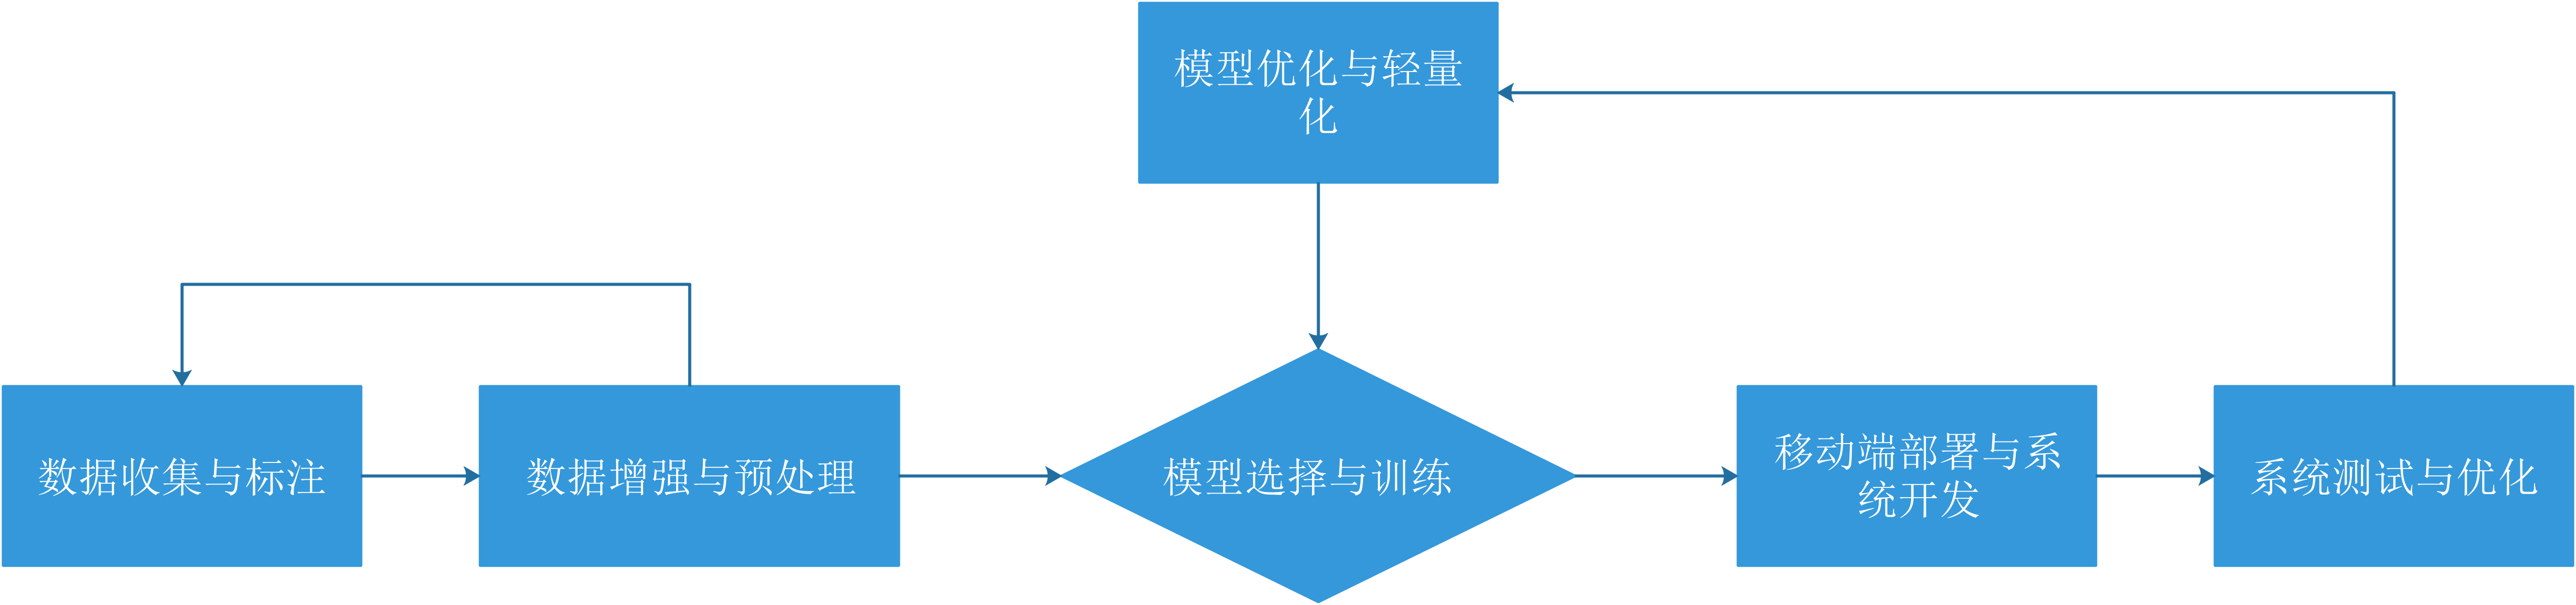
\includegraphics[width=\textwidth]{pictures/技术路线图.png}
  \caption{技术路线图}
  \label{fig:tec_road}
\end{figure}

\subsection{工具选型}
\subsubsection{PyTorch}
PyTorch作为一款深度学习框架,因其采用Python语言编写且支持动态图计算而备受青睐。基于动态图的特性,研究者能够灵活地在网络运行时调整模型结构,对于快速验证新想法、实现自定义算子非常方便。此外,PyTorch社区活跃度高,相关教程、插件、示例众多,能够在开发中快速获得技术支持。然而,PyTorch的动态图机制在一定程度上也会增加内存开销,对于资源受限的环境需要进行深度优化才能稳定运行。同时,PyTorch在移动端或嵌入式部署上仍需借助其他工具(如TorchScript、ONNX等)进行适配,部分新算子的转换和跨平台兼容尚不完善。与部分更注重大规模分布式训练的框架相比,PyTorch在极端场景下的性能也可能稍逊一筹,因此必须结合项目规模和硬件环境综合考量。

在本项目中,使用 PyTorch 搭建灵活的深度学习管线,借助动态图机制方便地实现自定义网络结构,并在多 GPU 并行训练的支持下加速模型迭代与性能优化。

\subsubsection{PyCharm}
PyCharm是专为Python语言设计的集成开发环境,提供了成熟的代码补全、版本控制、单元测试和调试功能,能显著提升开发效率与可维护性。它对Python包管理和虚拟环境有良好支持,易于在大型深度学习项目中配置依赖和管理模块。借助PyCharm的可视化调试,研究者能更直观地追踪网络参数变化和中间结果,有助于快速定位错误。另一方面,PyCharm由于功能丰富,运行时资源开销相对较大,尤其在硬件配置不高的设备上,可能会出现卡顿或加载缓慢等现象。同时,PyCharm虽然能通过插件兼容多语言,但真正能充分发挥其能力的还是Python生态,对于其他语言或跨平台开发的支持并不如专门工具完善。

在本项目中,使用 PyCharm 作为主要的 Python 开发环境,它提供了完善的调试、版本控制和单元测试功能,助力团队快速搭建并维护深度学习项目的开发流程。

\subsubsection{NVIDIA GPU}
NVIDIA GPU以强大的并行计算能力为深度学习训练和推理提供了硬件基础,结合CUDA、cuDNN等工具链能够显著缩短模型训练时间,并支持多卡分布式训练。成熟的硬件与软件生态,让研究者能在相对短的时间内构建大规模神经网络并进行快速迭代。然而,NVIDIA GPU的购置成本和使用成本均较高,功耗大且对散热要求高,适合在专业实验室或数据中心环境中使用。对于预算较紧、规模较小的团队,可能难以承受高端GPU的采购和维护费用。另外,当前深度学习主流框架大多对NVIDIA GPU优化较好,但若须迁移至其他GPU或专用AI加速芯片,则需要对软件栈进行相应改造,缺乏统一的解决方案也是一个局限性。

在本项目中,借助 NVIDIA GPU 强大的并行计算能力来加速模型训练与推理,大幅缩短了深度学习模型的开发周期并增强了实用性能。

\subsubsection{LabelImg}
LabelImg,是一款轻量化的图像标注工具,界面简洁且上手容易,研究人员能够在其提供的可视化环境中快速绘制目标边界框并添加相应标签,显著降低了数据标注的门槛与成本。该工具能够生成通用的标注文件格式(如VOC或YOLO),从而与主流深度学习框架直接对接,不过它在处理大批量图像时仍依赖人工操作,对高度复杂的分割标注或多类别情形也可能显得不足,并且仍需引入人工复核流程来确保标注质量的一致性与准确性。

在本项目中,选择使用LabelImg来快速完成对病害图像的手动标注和边界框绘制,以高效率、低成本地获得高质量数据,为后续模型训练和评估提供可靠的标签支持。

\subsubsection{ONNX}
ONNX(Open Neural Network Exchange)是一个通用的模型交换格式,能在PyTorch、TensorFlow等不同框架间传递模型,对于多平台部署和工程应用而言大大简化了流程。研究者可以将模型转换为ONNX后,再利用如TensorRT、OpenVINO等推理引擎进行跨平台加速与优化。然而,ONNX在支持部分新兴或自定义算子时仍不够完善,遇到尚未纳入标准或高阶算子的场景,可能需要手动实现转换逻辑。此外,不同推理引擎对ONNX的优化程度不尽相同,同一个模型在不同平台的推理速度和内存占用会有明显差异,需要反复调试。对于网络结构复杂、包含很多自定义层的模型,ONNX转换过程也容易出现推理不一致或报错,定位并修复问题往往需要较多经验。

在本项目中,利用 ONNX 作为跨框架的模型交换格式,实现了从 PyTorch 到多种推理引擎的便捷转换与部署,显著简化了模型跨平台应用的流程。

\subsubsection{uni-app}
uni-app采用Vue.js技术栈,让开发者仅需一套代码即可发布至微信小程序、H5、App等多端,极大地提升了开发效率和应用一致性。依赖完善的插件生态,uni-app能快速集成常见功能,帮助项目更快实现前端交互逻辑、页面布局与移动端特性,对前端开发者尤其友好。然而,由于需要兼顾多端兼容,uni-app在底层性能和原生功能支持方面存在一定限制,在大型应用或需要大量硬件调用的场景下,需要以插件或自定义原生模块的形式实现。

在本项目中,采用 uni-app 搭建前端界面,一套代码即可发布到微信小程序和其他多端平台,有效减少了兼容性适配和重复开发的工作量。

\subsubsection{HbuilderX}
HBuilderX是与uni-app同源的前端开发工具,针对uni-app项目流程进行深度集成,拥有对项目结构、打包、预览等多项便捷支持。它启动速度较快,对uni-app的调试与编译优化做得较为彻底,云真机测试功能也大大缩减了多端测试的门槛。然而,与较通用的开发工具(如VS Code、WebStorm等)相比,HBuilderX的插件生态和扩展能力还相对有限,对于前端以外的其他语言支持也并不完善。开发者若有个性化的构建需求或跨语言项目需求,就需要在HBuilderX内编写额外脚本或配置文件,理解并掌握其内部打包流程。相对封闭的生态环境意味着在高度自定义场景中,可能会遇到更多技术性挑战和适配成本。

在本项目中,使用 HBuilderX 与 uni-app 深度集成的特点来加速调试和部署流程,并凭借其轻量化特性实现了多端真机预览,提高了前端开发的效率。

\subsection{研究思路}
\subsubsection{数据收集与标注}
植物病害检测的首要任务是构建高质量、多样化的数据集,以支撑模型的训练与优化。数据收集的全面性和标注的精确性直接决定了模型的识别能力与泛化水平。因此,本研究将在广泛的数据源基础上,构建一个全面覆盖不同农作物病害类型和发展阶段的病害图像数据库。

数据收集将分为三个主要方向:一是整合已有公开数据集,如PlantVillage、AI Challenger和Kaggle等,这些数据集涵盖大量不同作物的病害图像,具有较高的标注质量和代表性;二是网络爬取和合作收集,借助爬虫技术从农业网站和科研论文中获取病害图像,并与农业院校合作,共享病害影像资源。

标注是数据质量提升的重要环节,直接关系到模型对病害区域的精确定位和分类能力。本研究将使用LabelImg、VGG Image Annotator(VIA)等开源工具对收集到的图像进行逐一标注,标注内容包括病害类别、病变区域和病害程度等。最终的数据集将涵盖五种以上主要农作物病害,每种病害数据量不少于100条,总体数据集规模将超过1000条图像。

\subsubsection{数据预处理}
数据预处理旨在提升模型对复杂环境的适应能力,减少因数据质量不佳而导致的训练偏差。预处理环节将针对数据的多样性和均衡性进行系统化处理,确保模型能够学习到病害区域的关键特征。

首先,图像增强技术将在数据扩展中发挥重要作用。通过随机旋转、翻转、亮度调整、裁剪和缩放等方法,生成多种角度和光照条件下的病害图像,增强模型的稳定性。此外,将添加噪声和颜色扰动,使模型对不同光线和环境条件下的病害表现更加敏感,避免模型对特定特征的过拟合。

尺寸归一化也是预处理的重要部分,为确保输入模型的图像一致性,将所有图像调整至224x224或256x256标准尺寸,这有助于模型收敛并提升训练速度。同时,数据清洗将在整个过程中穿插进行,剔除模糊、重复以及明显不符合标准的图像,确保数据集的高质量。

类别平衡问题将在预处理中重点解决,针对某些稀缺类别病害图像,通过生成对抗网络(GAN)扩展数据集,弥补少样本类别的不足,提升模型对小样本病害的识别能力。同时,对多样本类别进行下采样,防止模型训练过程中偏向于数据量较多的类别。

主要的数据预处理具体流程如图\ref{fig:data_preprocessing}:

\begin{figure}[H]
	\centering
	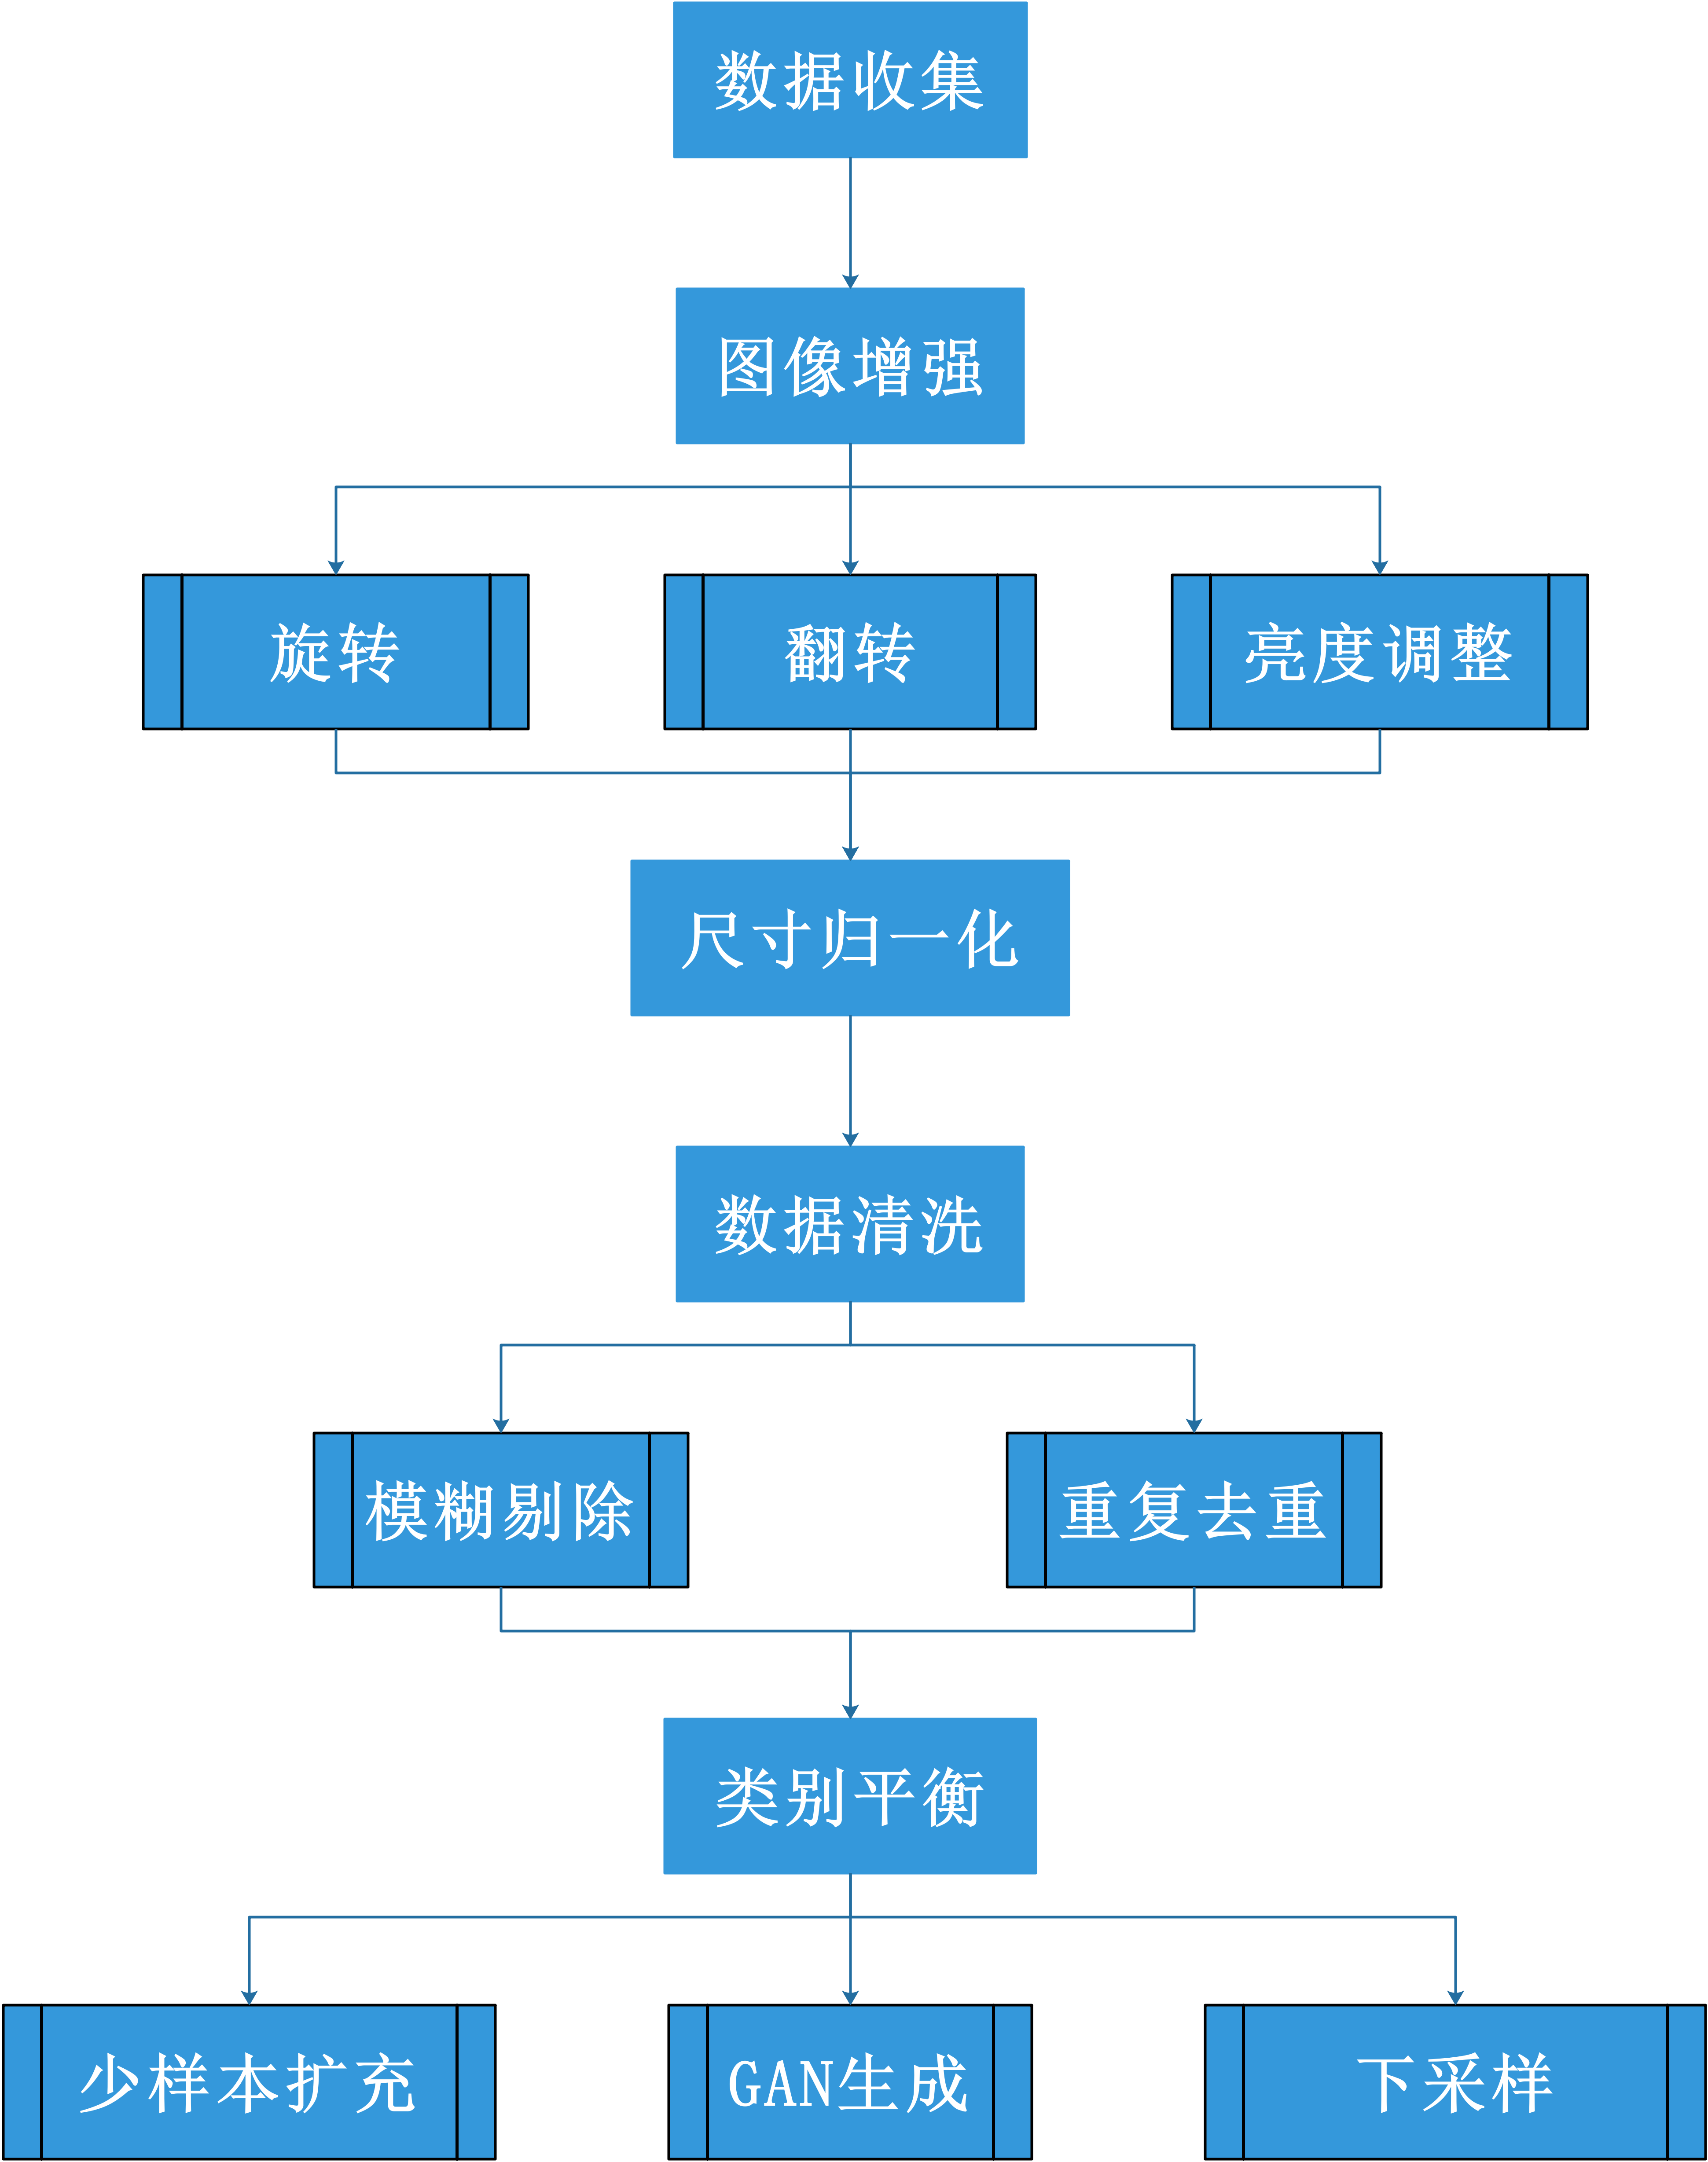
\includegraphics[width=0.5\textwidth]{pictures/数据预处理流程图.png}
	\caption{数据预处理流程图}
	\label{fig:data_preprocessing}
\end{figure}


\subsubsection{选择合适的模型进行训练}
模型选择将直接影响最终系统的检测精度和响应速度。本研究将在主流深度学习架构的基础上进行模型筛选,主要涵盖两大类模型:卷积神经网络(CNN)和基于Transformer的模型。

在卷积神经网络方面,将选择ResNet、MobileNet和DenseNet等经典架构进行对比。ResNet凭借残差连接有效解决了深层网络的梯度消失问题,在复杂场景下表现优异;MobileNet以其轻量化结构适合移动端部署,能够在保持较高检测精度的同时减少计算成本;DenseNet通过特征传递机制,减少冗余参数,适合小样本病害检测任务。

在Transformer模型方面,将重点评估Vision Transformer(ViT)和Swin Transformer。这些模型在大规模数据集上的优异表现表明,Transformer架构在视觉任务中具有强大的特征提取和多目标检测能力。ViT通过自注意力机制捕捉病害区域的全局特征,适合复杂背景和多目标任务;Swin Transformer采用分层滑动窗口机制,能够有效提升病害检测的精度和稳定性。

\subsubsection{模型优化}
模型优化是提升检测精度和运行效率的重要阶段,涉及到模型在不同平台上的适配和轻量化处理。本研究将通过迁移学习、数据增强和模型压缩等方式,进一步提升模型性能。

迁移学习将成为优化过程中的重要策略,通过在ImageNet等大型数据集上预训练模型,再在植物病害数据集上进行微调,使模型能够更快收敛并提升检测精度。此外,通过L2正则化和Dropout等正则化技术,减少模型复杂度,有效防止过拟合。

模型剪枝和量化也是轻量化处理的核心环节。剪枝将移除对检测结果贡献较小的神经元或网络层,从而减少模型的参数量;量化将模型权重从32位浮点数转换为8位整数,进一步降低存储需求和计算成本。在此基础上,知识蒸馏将复杂模型的知识迁移到轻量级学生模型,使其在减少体积的同时保持较高的检测精度。

优化完成后,模型将导出为轻量化的ONNX格式,以便部署至小程序中,实现病害检测的实际应用。

\subsubsection{小程序系统开发}
模型训练完成后,模型将被集成至微信小程序中,实现病害检测的实际应用。系统开发将围绕用户体验和功能需求展开,确保最终系统具备高效、便捷和实用的特点。

在系统开发方面,将使用uni-app等框架构建小程序前端界面,用户能够通过简单的交互界面上传作物图像,模型将完成病害检测并返回结果。系统将支持图像拍摄上传、实时检测和结果反馈等功能,用户能够快速获得病害诊断信息。

系统还将具备病害历史记录管理功能,帮助用户追踪病害的发展情况。此外,小程序将支持离线运行,通过将模型直接集成至移动设备,实现田间无网络环境下的离线病害检测。

\subsection{预期研究成果}
\subsubsection{高质量的数据集}
本研究将构建涵盖五种以上主要农作物病害的高质量图像数据集。该数据集不仅包含不同病害类型的高分辨率图像,还会涵盖多地域、多生长周期以及多场景的样本,以保证数据多样性和代表性。所有图像均会进行专业标注,包括病害类型、病变区域以及病害程度等细粒度标签,为后续模型训练提供精确的监督信息。同时,数据在采集和标注环节会遵循法律和隐私保护要求,并确保标注一致性与准确性。最终,经过清洗和增强后的数据集将成为植物病害检测的重要资源,为后续的模型研究与扩展应用奠定坚实基础。
\subsubsection{高精度、健壮的植物病害检测模型}
本项目将研发适用于移动端及多平台部署的深度学习模型。首先,基于卷积神经网络与新兴的 Transformer 架构,对比多种主流网络(如 ResNet、DenseNet、MobileNet、Vision Transformer 等),借助迁移学习和数据增强在植物病害数据集上进行针对性微调;然后,结合剪枝、量化与知识蒸馏等技术对模型进行轻量化优化,确保在资源受限的移动设备上也能实现实时推理。最终模型将具备对多种病害类型的高精度识别和健壮性,且在推理速度与模型大小上达到可实际应用的水平。
\subsubsection{易用的植物病害检测移动应用}
在应用层面,将面向微信小程序实现农田病害检测功能,用户只需通过手机拍照或上传图像,即可实时获得病害识别结果和防控建议。为了满足实际农田环境对离线检测的需求,应用会支持断网使用,并提供可离线运行的简化模型。同时还将设计简洁的用户交互界面,集成病害历史记录管理与统计分析模块,使农业生产者能追踪病害趋势并及时采取防控措施。通过与农技服务平台或农业管理系统的对接,有望形成完整的“检测-诊断-管理”闭环,为智慧农业与精准农作提供有效支撑。
\subsubsection{经济与社会效益}
提高农田病害检测效率、降低人力投入、减少农药浪费。加强对疾病早期识别和预防,保障农产品质量与产量。推动农业信息化与数字化,提升农村经济发展水平,对智慧农业和精准农业具有示范意义。

\section{研究工作计划}
\begin{longtblr}[
    theme=plain,
    entry=none,
  ]{
    colspec = {|X[2,l]|X[3,l]|},
    row{1} = {c},
    hlines
  }
    起止时间 & 内容 \\
    2024-11-05 - 2024-12-20 & 查阅文献,撰写文献综述,外文翻译,完成调研 \\
    2024-12-21 - 2025-01-08 & 开题报告的撰写和开题报告答辩 \\
    2025-01-09 - 2025-01-31 & 数据分析和前期处理 \\
    2025-02-01 - 2025-03-22 & 检测模型设计和分析,模型构建和导出 \\
    2025-03-18 - 2025-03-22 & 中期检查 \\
    2025-03-23 - 2025-04-20 & 模型完善、软件设计 \\
    2025-04-21 - 2025-05-07 & 毕业论文撰写 \\
    2025-05-08 - 2025-05-16 & 教师评阅 \\
    2025-05-17前 & 毕业设计答辩 \\
  \end{longtblr}
  